% Section 6: Release Planning
\section{Release Planning}

The release planning uses Sprint Based Agile Release Planning, organizing prioritized requirements into release backlogs and development sprints for iterative delivery.

\subsection{Release Planning Technique: Sprint Based Agile Planning}

\subsubsection{Description}

Sprint Based Agile Release Planning is a technique commonly used in agile software development methodologies such as Scrum. The process involves:

\begin{enumerate}
    \item \textbf{Product Backlog}: A prioritized list of all requirements for the product.
    \item \textbf{Release Backlog}: A subset of the product backlog selected for a specific release, based on business value, dependencies, and capacity.
    \item \textbf{Sprint Planning}: Requirements from the release backlog are allocated to fixed length development sprints (typically 1 to 4 weeks).
    \item \textbf{Sprint Execution}: The development team implements the requirements assigned to each sprint.
\end{enumerate}

Each sprint produces a potentially shippable product increment, allowing for early validation and feedback.

\subsubsection{Planning Approach and Assumptions}

The release planning for CookWise follows Sprint-Based Agile principles with the following approach:

\textbf{Sprint Planning Process:}
\begin{enumerate}
    \item \textbf{Backlog Refinement}: Prior to each sprint, the team reviews the prioritized product backlog (from Section 5), breaks down high-level requirements into implementable tasks, and estimates effort using story points.
    \item \textbf{Velocity Estimation}: Team velocity is estimated at 12-16 story points per sprint based on a 4-person team. Initial sprints may have lower velocity (8-10 points) as the team establishes development workflows.
    \item \textbf{Requirement Selection}: Requirements are selected for each sprint based on: (a) business priority from 100-dollar test, (b) technical dependencies, (c) team capacity, and (d) balanced mix of domain, product, data, and quality requirements.
    \item \textbf{Sprint Review and Adaptation}: At the end of each sprint, delivered functionality is reviewed. If velocity differs from estimates, subsequent sprint plans are adjusted accordingly.
\end{enumerate}

\vspace{0.3cm}

\textbf{Planning Assumptions:}
\begin{itemize}
    \item \textbf{Sprint Duration}: Each sprint is 2 weeks long (10 working days).
    \item \textbf{Sprints per Release}: Each release consists of 3 sprints (6 weeks total per release).
    \item \textbf{Team Composition}: Development team consists of 4 members (2 full-stack developers, 1 backend specialist, 1 frontend specialist).
    \item \textbf{Team Capacity}: The team can implement 3 to 4 requirements per sprint, depending on requirement complexity and technical dependencies. Complex requirements (e.g., web scraping, AI integration) count as 2-3 simpler requirements in terms of effort.
    \item \textbf{Velocity Tracking}: Story points assigned to each requirement type: Domain requirements (2-3 points), Product requirements (2-4 points), Data requirements (1-2 points), Quality requirements (3-5 points for implementation and testing).
    \item \textbf{Release Frequency}: Release 1.0 is the minimum viable product (MVP) targeted for initial market launch. Release 2.0 follows 6 weeks after Release 1.0 launch, adding enhanced functionality.
    \item \textbf{Technical Dependencies}: Requirements with dependencies must be implemented in the correct order (foundational requirements before dependent features). Dependency analysis performed during backlog refinement ensures proper sequencing.
    \item \textbf{Testing Integration}: Each sprint includes unit testing, integration testing, and quality validation (for QRs). No separate testing phase - testing is integrated throughout each sprint.
\end{itemize}

\subsection{Release 1.0: Minimum Viable Product}

\subsubsection{Release Goals}

Release 1.0 delivers the core value proposition: sale based recipe suggestions and automatic shopping list generation. This release implements the 9 Must Have requirements identified in Section 5, establishing foundational infrastructure, implementing core functionality, and ensuring acceptable performance and data accuracy.

\subsubsection{Release 1.0 Backlog}

Table \ref{tab:release1backlog} shows the requirements selected for Release 1.0, organized by priority.

\begin{table}[htbp]
\centering
\caption{Release 1.0 Backlog}
\label{tab:release1backlog}
\begin{tabular}{|l|l|l|}
\hline
\textbf{ID} & \textbf{Requirement} & \textbf{Type} \\
\hline
DL1 & Web scraping for product and pricing data & Domain \\
\hline
DL2 & GDPR compliance for user and partner data & Domain \\
\hline
DR1 & Core entity data models & Data \\
\hline
DR2 & Relationship and associative entity data models & Data \\
\hline
PR1 & Sale based recipe suggestions & Product \\
\hline
PR2 & Recipe search and filtering & Product \\
\hline
PR3 & Automatic grocery shopping list generation & Product \\
\hline
QR1 & Performance: Recipe generation response time & Quality \\
\hline
QR3 & Accuracy: Price data correctness & Quality \\
\hline
\end{tabular}
\end{table}

\subsubsection{Sprint Allocation for Release 1.0}

The 9 requirements in Release 1.0 are distributed across 3 sprints, considering technical dependencies and implementation effort. Table \ref{tab:release1sprints} presents the sprint allocation.

\begin{table}[htbp]
\centering
\caption{Release 1.0 Sprint Allocation}
\label{tab:release1sprints}
\begin{tabular}{|l|l|l|}
\hline
\textbf{Sprint} & \textbf{Requirements} & \textbf{Focus} \\
\hline
\textbf{Sprint 1} & DL1: Web scraping & Foundation \\
(Weeks 1-2) & DL2: GDPR compliance & \\
 & DR2: Relationship data models & \\
\hline
\textbf{Sprint 2} & DR1: Core entity data models & Core Data \\
(Weeks 3-4) & PR2: Recipe search and filtering & \\
 & QR3: Accuracy validation & \\
\hline
\textbf{Sprint 3} & PR1: Sale based recipe suggestions & Core Features \\
(Weeks 5-6) & PR3: Shopping list generation & \\
 & QR1: Performance optimization & \\
\hline
\end{tabular}
\end{table}

\textbf{Sprint 1 (Foundation):} Establishes foundational infrastructure with DL1 (Web scraping), DL2 (GDPR compliance), and DR2 (Relationship data models).

\vspace{0.2cm}
\textbf{Sprint 2 (Core Data):} Implements database structure with DR1 (Core entity data models), PR2 (Recipe search and filtering), and QR3 (Accuracy validation).

\vspace{0.2cm}
\textbf{Sprint 3 (Core Features):} Delivers primary value proposition with PR1 (Sale based recipe suggestions), PR3 (Shopping list generation), and QR1 (Performance optimization).

\subsubsection{Release 1.0 Dependencies}

Figure \ref{fig:release1deps} illustrates the key dependencies between requirements in Release 1.0. Arrows indicate that one requirement depends on another being implemented first.

\begin{figure}[htbp]
\centering
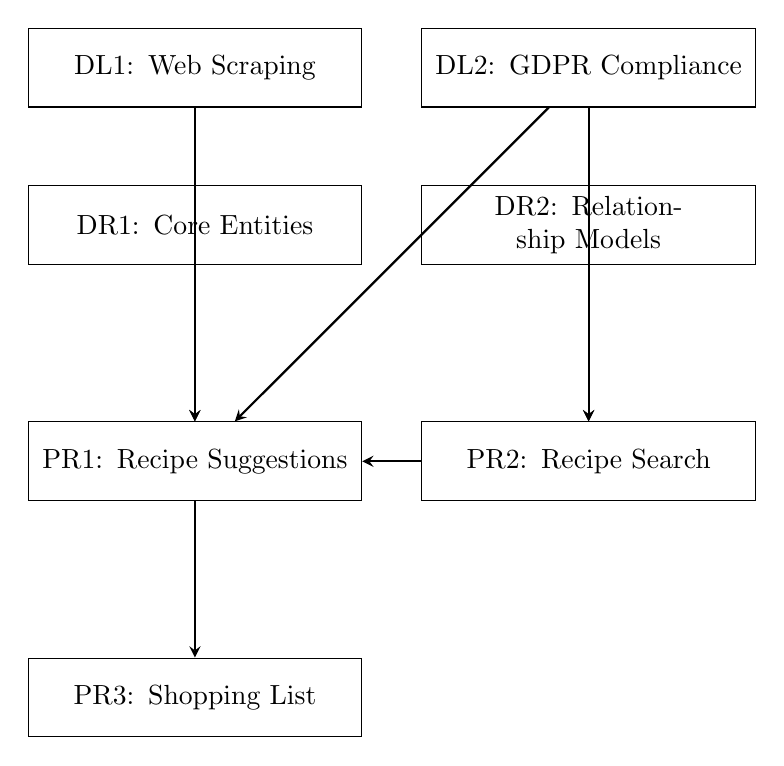
\begin{tikzpicture}[node distance=2cm]
\tikzstyle{req} = [rectangle, draw, text width=4cm, text centered, minimum height=1cm]
\tikzstyle{arrow} = [thick,->,>=stealth]

\node (dl1) [req] {DL1: Web Scraping};
\node (dl2) [req, right of=dl1, xshift=3cm] {DL2: GDPR Compliance};
\node (dr2) [req, below of=dl2] {DR2: Relationship Models};
\node (dr1) [req, below of=dl1] {DR1: Core Entities};
\node (pr2) [req, below of=dr2, yshift=-1cm] {PR2: Recipe Search};
\node (pr1) [req, below of=dr1, yshift=-1cm] {PR1: Recipe Suggestions};
\node (pr3) [req, below of=pr1, yshift=-1cm] {PR3: Shopping List};

\draw [arrow] (dl1) -- (pr1);
\draw [arrow] (dl2) -- (pr2);
\draw [arrow] (dl2) -- (pr1);
\draw [arrow] (dr2) -- (pr2);
\draw [arrow] (dr1) -- (pr1);
\draw [arrow] (pr2) -- (pr1);
\draw [arrow] (pr1) -- (pr3);

\end{tikzpicture}
\caption{Release 1.0 Requirement Dependencies}
\label{fig:release1deps}
\end{figure}

\subsection{Release 2.0: Enhanced User Experience}

\subsubsection{Release Goals}

Release 2.0 enhances user experience through personalization, usability improvements, and expanded data features. This release implements 10 Should Have requirements from Section 5, differentiating CookWise from basic recipe apps and increasing user engagement.

\subsubsection{Release 2.0 Backlog}

Table \ref{tab:release2backlog} shows the requirements selected for Release 2.0.

\begin{table}[htbp]
\centering
\caption{Release 2.0 Backlog}
\label{tab:release2backlog}
\begin{tabular}{|l|l|l|}
\hline
\textbf{ID} & \textbf{Requirement} & \textbf{Type} \\
\hline
DL3 & Shopping list and meal planning system & Domain \\
\hline
DR3 & User profile and preference data & Data \\
\hline
DR4 & Recipe nutritional information & Data \\
\hline
DR5 & Retailer store location data & Data \\
\hline
PR4 & Personalized recipe recommendations & Product \\
\hline
PR5 & Dietary preference and restriction filters & Product \\
\hline
PR6 & Price comparison across multiple retailers & Product \\
\hline
PR7 & Shopping list modification and sharing & Product \\
\hline
QR2 & Usability: First recipe selection time & Quality \\
\hline
QR4 & Scalability: Concurrent user capacity & Quality \\
\hline
\end{tabular}
\end{table}

\subsubsection{Sprint Allocation for Release 2.0}

The 10 requirements in Release 2.0 are distributed across 3 sprints. Table \ref{tab:release2sprints} presents the sprint allocation.

\begin{table}[htbp]
\centering
\caption{Release 2.0 Sprint Allocation}
\label{tab:release2sprints}
\begin{tabular}{|l|l|l|}
\hline
\textbf{Sprint} & \textbf{Requirements} & \textbf{Focus} \\
\hline
\textbf{Sprint 4} & DR3: User profiles and preferences & Personalization \\
(Weeks 7-8) & PR5: Dietary filters & \\
 & DR4: Nutritional information & \\
\hline
\textbf{Sprint 5} & PR4: Personalized recommendations & Enhanced \\
(Weeks 9-10) & DL3: Meal planning system & Features \\
 & PR7: List modification and sharing & \\
 & QR2: Usability improvements & \\
\hline
\textbf{Sprint 6} & DR5: Store location data & Data \\
(Weeks 11-12) & PR6: Price comparison & Expansion \\
 & QR4: Scalability improvements & \\
\hline
\end{tabular}
\end{table}

\vspace{0.2cm}
\textbf{Sprint 4 (Personalization):} Introduces personalization with DR3 (User profiles), PR5 (Dietary filters), and DR4 (Nutritional information).

\vspace{0.2cm}
\textbf{Sprint 5 (Enhanced Features):} Implements advanced features with PR4 (Personalized recommendations), DL3 (Meal planning), PR7 (List modification and sharing), and QR2 (Usability improvements).

\vspace{0.2cm}
\textbf{Sprint 6 (Data Expansion):} Expands available data with DR5 (Store location data), PR6 (Price comparison), and QR4 (Scalability improvements).

\subsection{Product Backlog and Future Releases}

After Release 2.0, the remaining 14 requirements from Section 5 form the backlog for future releases. Table \ref{tab:futurebacklog} categorizes these requirements.

\begin{table}[htbp]
\centering
\caption{Future Release Backlog}
\label{tab:futurebacklog}
\begin{tabular}{|l|l|l|}
\hline
\textbf{Priority} & \textbf{Requirements} & \textbf{Count} \\
\hline
\textbf{Could Have} & DL4, DR6, DR7, DR8, PR8, PR9, PR12, QR5 & 8 \\
(Release 3.0) & & \\
\hline
\textbf{Won't Have} & DR9, DR10, PR10, PR11, PR13, PR14 & 6 \\
(Release 4.0+) & & \\
\hline
\end{tabular}
\end{table}

The Could Have requirements would be considered for Release 3.0, while Won't Have requirements are deferred to Release 4.0 or later based on market feedback and available resources.

\subsection{Release Timeline and Milestones}

Figure \ref{fig:timeline} presents the overall release timeline for CookWise, showing the progression from initial development through Release 2.0.

\begin{figure}[htbp]
\centering
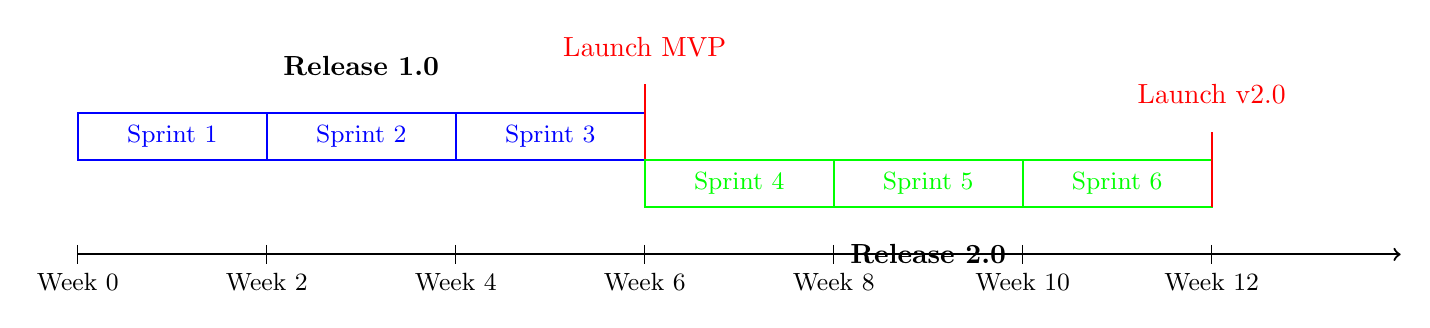
\begin{tikzpicture}[scale=1.2]
\draw[thick,->] (0,0) -- (14,0);
\foreach \x/\label in {0/Week 0, 2/Week 2, 4/Week 4, 6/Week 6, 8/Week 8, 10/Week 10, 12/Week 12}
    \draw (\x,0.1) -- (\x,-0.1) node[below] {\small \label};

\draw[thick, blue] (0,1) rectangle (2,1.5) node[pos=.5] {\small Sprint 1};
\draw[thick, blue] (2,1) rectangle (4,1.5) node[pos=.5] {\small Sprint 2};
\draw[thick, blue] (4,1) rectangle (6,1.5) node[pos=.5] {\small Sprint 3};
\node at (3,2) {\textbf{Release 1.0}};
\draw[thick, red] (6,1) -- (6,1.8);
\node[red] at (6,2.2) {Launch MVP};

\draw[thick, green] (6,0.5) rectangle (8,1) node[pos=.5] {\small Sprint 4};
\draw[thick, green] (8,0.5) rectangle (10,1) node[pos=.5] {\small Sprint 5};
\draw[thick, green] (10,0.5) rectangle (12,1) node[pos=.5] {\small Sprint 6};
\node at (9,0) {\textbf{Release 2.0}};
\draw[thick, red] (12,0.5) -- (12,1.3);
\node[red] at (12,1.7) {Launch v2.0};

\end{tikzpicture}
\caption{CookWise Release Timeline}
\label{fig:timeline}
\end{figure}

The complete development and launch cycle spans 12 weeks: Release 1.0 MVP launches at Week 6, followed by Release 2.0 at Week 12.

\subsection{Risk Management and Mitigation}

Several risks could impact the release plan, and the following mitigation strategies have been identified:

\begin{itemize}
    \item \textbf{Web Scraping Reliability}: Retailers may change website structure. Mitigation includes robust error handling and planned API transition.

    \item \textbf{Recipe Quality and Coverage}: Initial database may lack variety. Mitigation includes partnerships with food bloggers and user testing.

    \item \textbf{Performance}: Recipe suggestions may not meet 5 second target. Mitigation includes dedicated optimization time and caching strategies.

    \item \textbf{User Adoption}: MVP may not provide sufficient value. Mitigation includes user testing and marketing materials highlighting cost savings.
\end{itemize}

\subsection{Success Metrics and Evaluation}

The success of each release will be evaluated using the following metrics:

\vspace{0.2cm}
\textbf{Release 1.0 Success Metrics:}
\begin{itemize}
    \item \textbf{User Acquisition}: 1,000 registered users within first month
    \item \textbf{User Engagement}: 60\% of users generate at least one shopping list within first week
    \item \textbf{Performance}: 95\% of recipe suggestions return within 5 seconds
    \item \textbf{Data Quality}: 95\% accuracy in price data as validated weekly
    \item \textbf{Technical Stability}: Less than 5\% error rate in web scraping operations
\end{itemize}

\vspace{0.2cm}
\textbf{Release 2.0 Success Metrics:}
\begin{itemize}
    \item \textbf{User Growth}: 3,000 total registered users by end of Release 2.0
    \item \textbf{Feature Adoption}: 40\% of users set dietary preferences within first week
    \item \textbf{Personalization Impact}: 30\% increase in recipe selection rate for users with completed profiles
    \item \textbf{User Satisfaction}: Average rating of 4.0 out of 5.0 for usability
    \item \textbf{System Scalability}: Support 300 concurrent users with acceptable performance
\end{itemize}

These metrics will be monitored continuously after each release launch. If metrics fall short of targets, the team will analyze user feedback and adjust the release plan accordingly. The flexibility of the sprint based approach allows for rapid iteration and course correction based on real world data.